\documentclass[./main.tex]{subfiles}

\begin{document}
\begin{abstract}
\normalsize\noindent
Nella seguente analisi si vuole affrontare un problema di classificazione di attività motorie, utilizzando dati sull'accelerazione a cui è sottoposto un cellulare. Particolare attenzione deve essere posta nell'identificare correttamente quando il cellulare viene agitato volontariamente ({\em shake}) o meno. Un campo applicativo per questo modello può essere un software per cellulare di monitoraggio di attività fisica, che integri delle funzionalità quando l'utente effettua uno {\em shake}. L'errata classificazione di un'attività come {\em shake} può essere fonte di disturbo per l'utente, in quanto verrebbero attivate delle funzionalità quando non richiesto.
\end{abstract}
\section{Raccolta dei dati}
I dati sono stati raccolti sullo stesso cellulare, in campioni di circa $\SI{2}{\min}$ per attività. Le attività sono state eseguite da persone diverse. La rilevazione dei dati è stata effettuata tramite l'applicazione \texttt{PhonePi}\cite{kumarPhonePiSampleServer2019}.\\
Si sono considerate le seguenti attività motorie e attività legate all\rq{}utilizzo quotidiano del cellulare:
\begin{enumerate}
	\item camminata con cellulare in mano;
	\item camminata con cellulare in tasca;
	\item corsa con cellulare in mano;
	\item corsa con cellulare in tasca;
	\item utilizzo a riposo (chiamate e scrittura di messaggi);
	\item salti sul posto;
	\item salita e discesa di scale;
	\item shake volontario.
\end{enumerate}
Per ciascuna classe, si dispone di misurazioni a intervalli di ampiezza $\Delta t = \SI{10}{ms}$ della quantità
$$
\vec{a}_t = \begin{pmatrix}
a_{xt}\\
a_{yt}\\
a_{zt}
\end{pmatrix}\,,
$$
accelerazione del cellulare rispetto agli assi cartesiani di riferimento dell'accelerometro. L'analisi è stata condotta sull'intensità dell'accelerazione $a_t = \|\vec{a}_t\|$, ignorando l'effetto di disturbo dell'accelerazione di gravità. Da ogni campione sono stati tolti i primi e gli ultimi sette secondi, considerando solo i dati per le attività ``a regime''.
In Figura~\ref{fig:esempio} sono riportati dei grafici di esempio dei dati raccolti.
\begin{figure}[H]
	\centering
	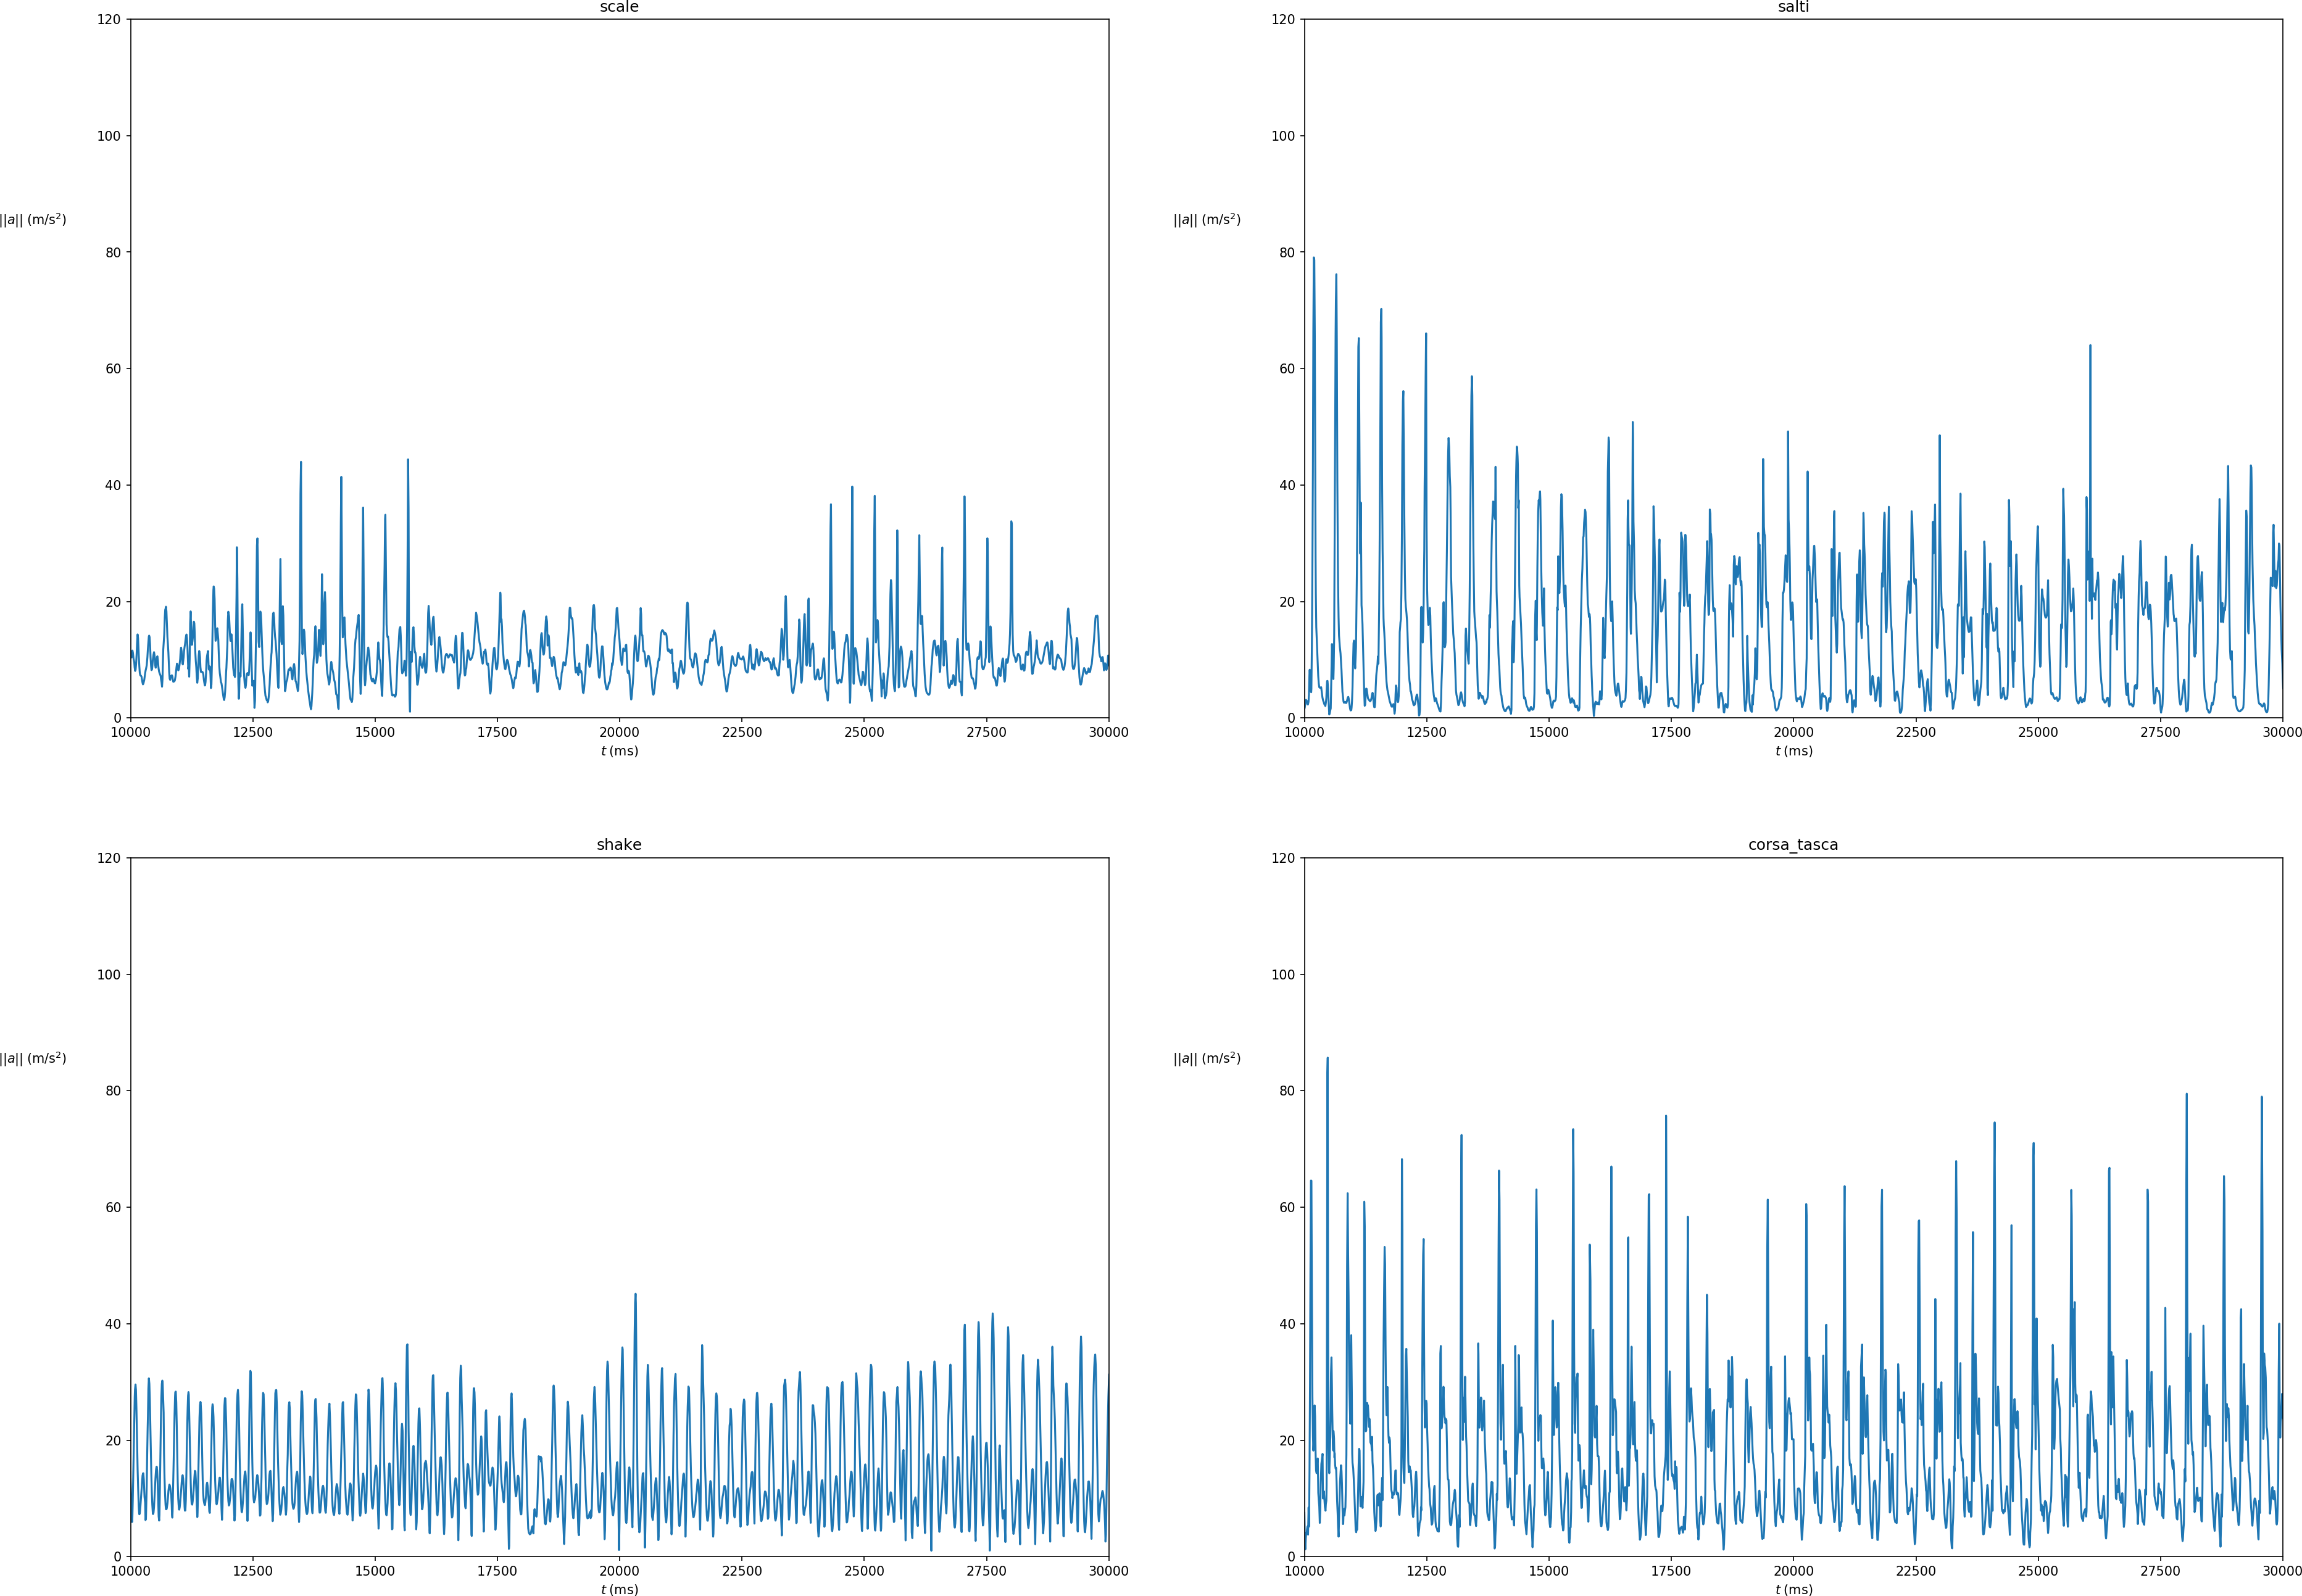
\includegraphics[width=.99\textwidth, keepaspectratio]{../../figure/espl.png}
	\caption{Intervalli $ [\SI{10}{\second}, \SI{30}{\second}] $ per le attività motorie di salita e discesa di scale, salti, shake, corsa con cellulare in tasca.}
	\label{fig:esempio}
\end{figure}
\end{document}